% Flowchart
% Author: Qrrbrbirlbel
\documentclass[tikz,border=10pt]{standalone}

\usetikzlibrary{shapes,backgrounds,calc,arrows}
\tikzset{>=stealth'}

\begin{document}

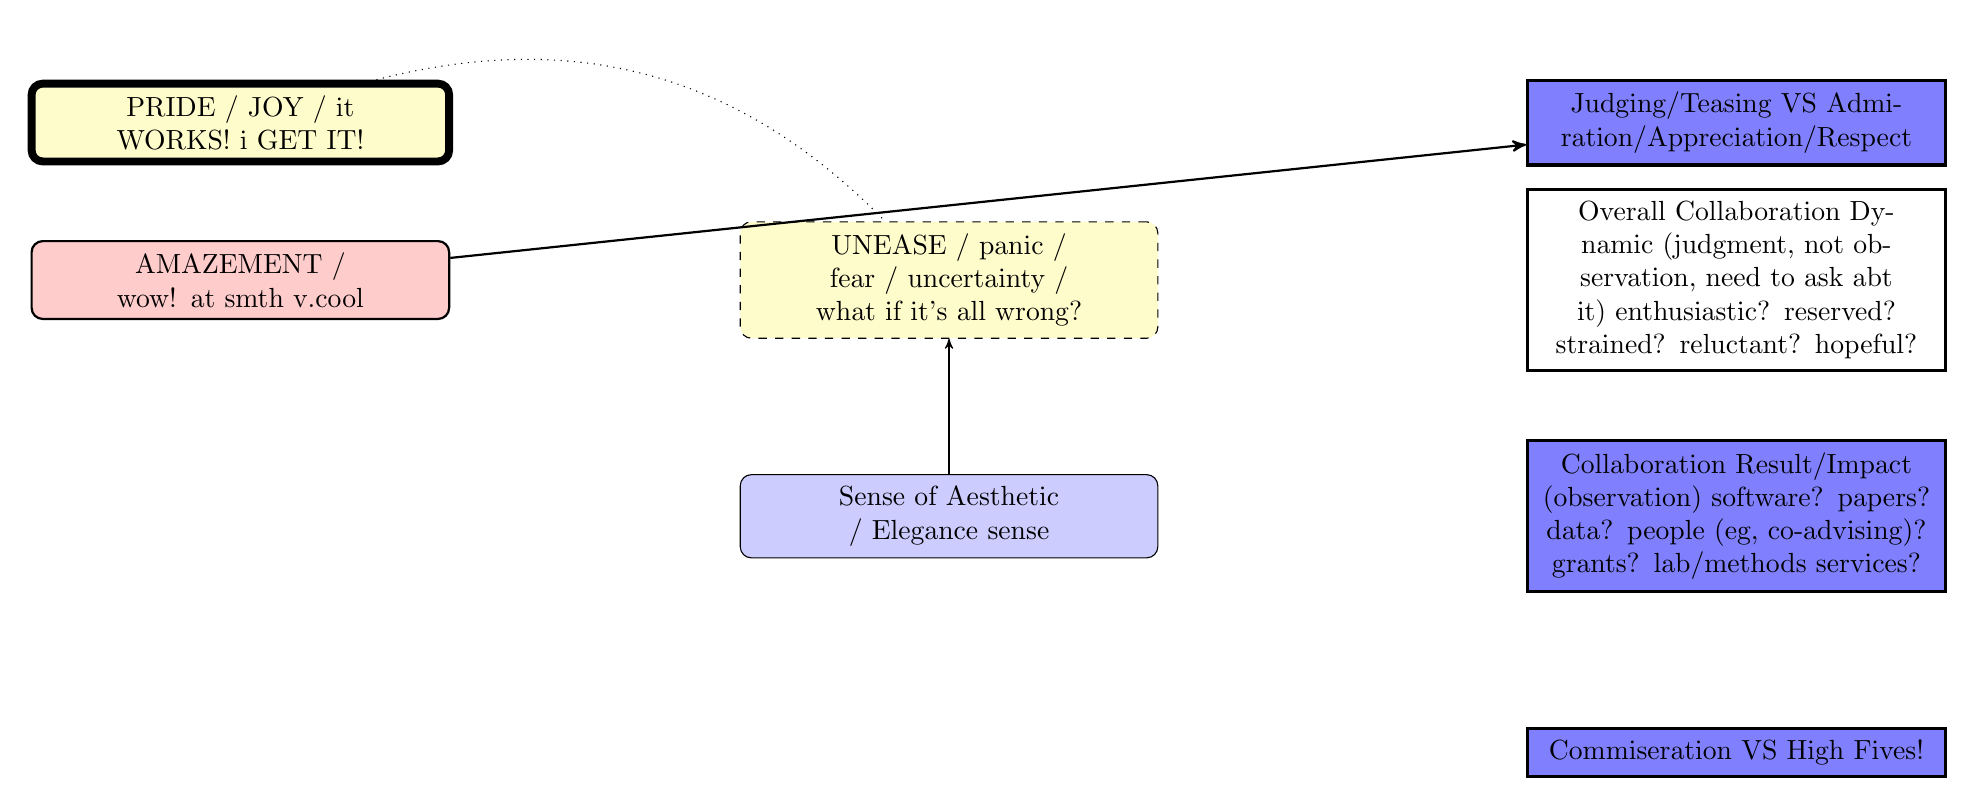
\begin{tikzpicture}

%% styles
\tikzstyle{bubble}=[draw, text centered, rounded corners, inner sep=1ex]

\tikzstyle{bumbox}=[draw, text centered, inner sep=1ex, very thick]

%% blobs
\node(P1)[text width=5cm, style = bubble, fill=blue!20] at (10, 0)
{
Sense of Aesthetic / Elegance sense
};

\node(P2)[text width=5cm, style = bubble, fill=yellow!20, dashed] at (10, 3)
{
UNEASE / panic / fear / uncertainty / what if it’s all wrong?
};

\node(P3)[text width=5cm, style = bubble, fill=red!20, thick] at (1, 3)
{
AMAZEMENT / wow! at smth v.cool
};

\node(P4)[text width=5cm, style = bubble, fill=yellow!20, line width=1mm] at (1, 5)
{
PRIDE / JOY / it WORKS! i GET IT!
};


%% text boxes

\node(O1)[text width=5cm, style = bumbox, fill=blue!50] at (20, 5)
{
Judging/Teasing VS Admiration/Appreciation/Respect
};

\node(O2)[text width=5cm, style = bumbox, fill=none] at (20, 3)
{
Overall Collaboration Dynamic (judgment, not observation, need to ask abt it)
enthusiastic? reserved? strained? reluctant? hopeful?
};

\node(O3)[text width=5cm, style = bumbox, fill=blue!50] at (20, 0)
{
Collaboration Result/Impact (observation)
software? papers? data? people (eg, co-advising)? grants? lab/methods services?
};

\node(O4)[text width=5cm, style = bumbox, fill=blue!50] at (20, -3)
{
Commiseration VS High Fives!
};

%% arrows


\path [draw, ->] (P1) -- (P2);

\path [draw] (P4) edge [bend left, dotted] (P2);

\path [draw, ->] (P3) edge [thick] (O1);

\end{tikzpicture}


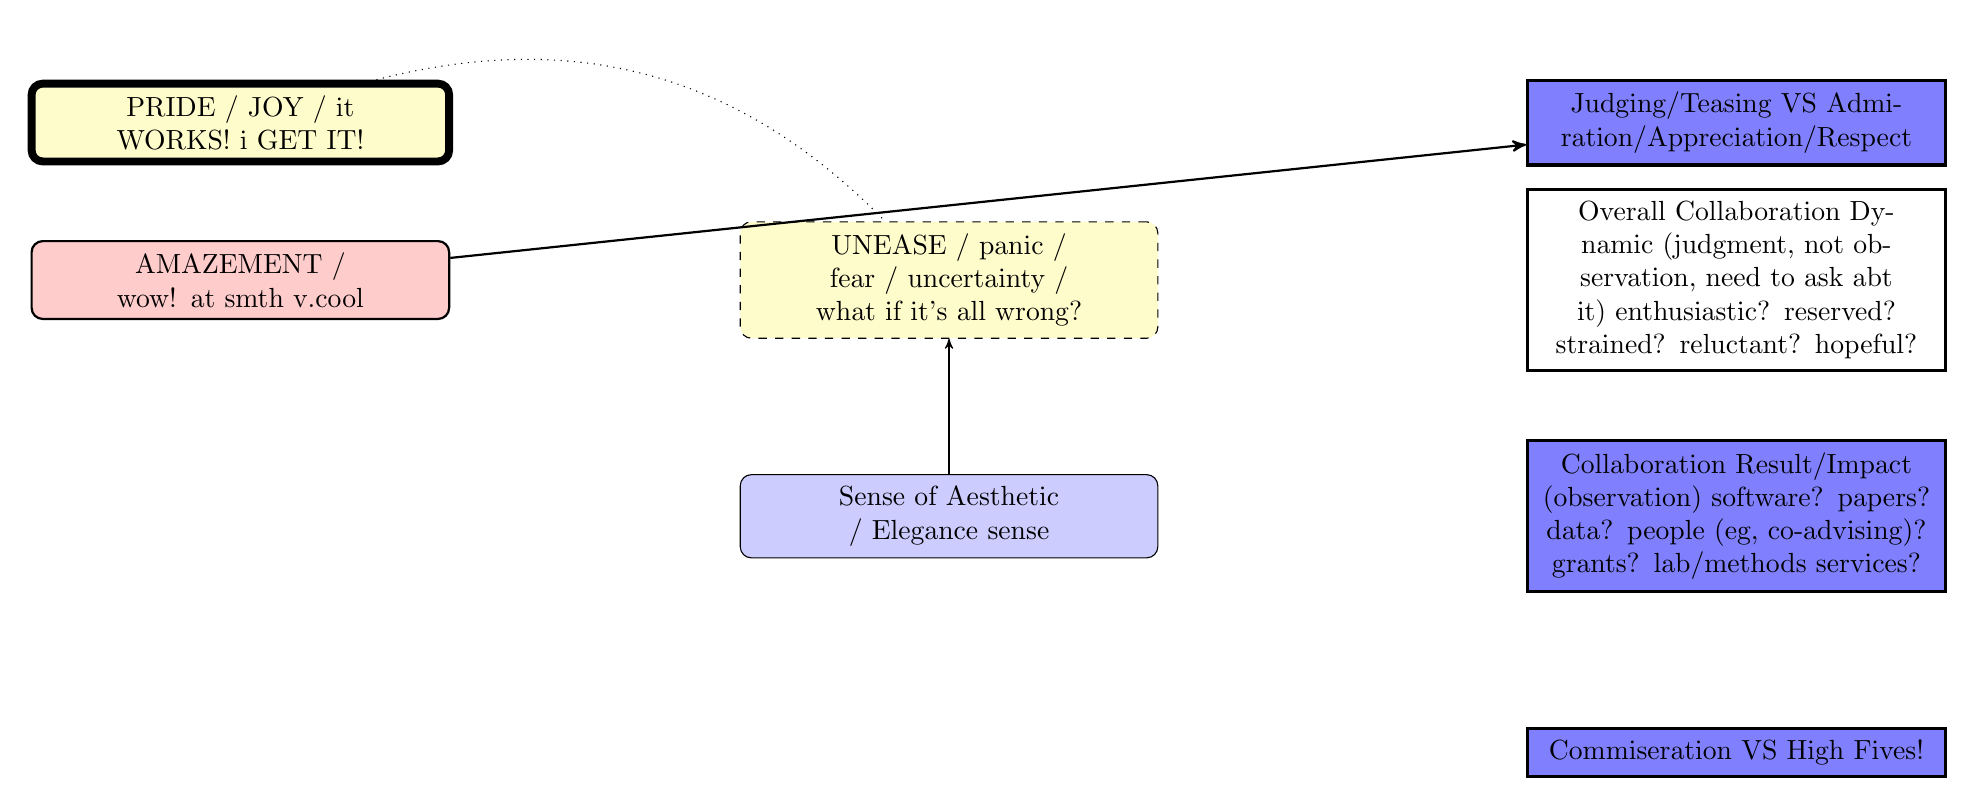
\begin{tikzpicture}

%% styles
\tikzstyle{bubble}=[draw, text centered, rounded corners, inner sep=1ex]

\tikzstyle{bumbox}=[draw, text centered, inner sep=1ex, very thick]

%% blobs
\node(P1)[text width=5cm, style = bubble, fill=blue!20] at (10, 0)
{
Sense of Aesthetic / Elegance sense
};

\node(P2)[text width=5cm, style = bubble, fill=yellow!20, dashed] at (10, 3)
{
UNEASE / panic / fear / uncertainty / what if it’s all wrong?
};

\node(P3)[text width=5cm, style = bubble, fill=red!20, thick] at (1, 3)
{
AMAZEMENT / wow! at smth v.cool
};

\node(P4)[text width=5cm, style = bubble, fill=yellow!20, line width=1mm] at (1, 5)
{
PRIDE / JOY / it WORKS! i GET IT!
};


%% text boxes

\node(O1)[text width=5cm, style = bumbox, fill=blue!50] at (20, 5)
{
Judging/Teasing VS Admiration/Appreciation/Respect
};

\node(O2)[text width=5cm, style = bumbox, fill=none] at (20, 3)
{
Overall Collaboration Dynamic (judgment, not observation, need to ask abt it)
enthusiastic? reserved? strained? reluctant? hopeful?
};

\node(O3)[text width=5cm, style = bumbox, fill=blue!50] at (20, 0)
{
Collaboration Result/Impact (observation)
software? papers? data? people (eg, co-advising)? grants? lab/methods services?
};

\node(O4)[text width=5cm, style = bumbox, fill=blue!50] at (20, -3)
{
Commiseration VS High Fives!
};

%% arrows


\path [draw, ->] (P1) -- (P2);

\path [draw] (P4) edge [bend left, dotted] (P2);

\path [draw, ->] (P3) edge [thick] (O1);

\end{tikzpicture}
\end{document}
